\documentclass[11pt,a4paper,oneside]{report}


\usepackage{amsmath,amssymb,calc,ifthen}

\usepackage{float}
%\usepackage{cancel}

\usepackage[table,usenames,dvipsnames]{xcolor} % for coloured cells in tables

\usepackage{tikz}

% Allows us to click on links and references!

\usepackage{hyperref}
\hypersetup{
    colorlinks,
    citecolor=black,
    filecolor=black,
    linkcolor=black,
    urlcolor=black
}

% Nice package for plotting graphs
% See excellent guide:
% http://www.tug.org/TUGboat/tb31-1/tb97wright-pgfplots.pdf
\usetikzlibrary{plotmarks}
\usepackage{amsmath,graphicx}
\usepackage{epstopdf}
\usepackage[font=Large,labelfont=bf]{caption}
\usepackage{subcaption}

% highlight - useful for TODOs and similar
\usepackage{color}
\newcommand{\hilight}[1]{\colorbox{yellow}{#1}}

\newcommand\ci{\perp\!\!\!\perp} % perpendicular sign
\newcommand*\rfrac[2]{{}^{#1}\!/_{#2}} % diagonal fraction

\usepackage{listings}



% margin size
\usepackage[margin=1in]{geometry}

\tikzstyle{state}=[circle,thick,draw=black, align=center, minimum size=2.1cm,
inner sep=0]
\tikzstyle{vertex}=[circle,thick,draw=black]
\tikzstyle{terminal}=[rectangle,thick,draw=black]
\tikzstyle{edge} = [draw,thick]
\tikzstyle{lo} = [edge,dotted]
\tikzstyle{hi} = [edge]
\tikzstyle{trans} = [edge,->]


\definecolor{mygreen}{rgb}{0,0.6,0}
\definecolor{mygray}{rgb}{0.5,0.5,0.5}
\definecolor{mymauve}{rgb}{0.58,0,0.82}

\lstset{ %
  backgroundcolor=\color{white},   % choose the background color; you must add 
%\usepackage{color} or \usepackage{xcolor}
  basicstyle=\footnotesize,        % the size of the fonts that are used for the 
%code
  breakatwhitespace=false,         % sets if automatic breaks should only happen 
%at whitespace
  breaklines=true,                 % sets automatic line breaking
  captionpos=b,                    % sets the caption-position to bottom
  commentstyle=\color{mygreen},    % comment style
  deletekeywords={...},            % if you want to delete keywords from the 
%given language
  escapeinside={\%*}{*)},          % if you want to add LaTeX within your code
  extendedchars=true,              % lets you use non-ASCII characters; for 
%8-bits encodings only, does not work with UTF-8
  frame=single,                    % adds a frame around the code
  keepspaces=true,                 % keeps spaces in text, useful for keeping 
%indentation of code (possibly needs columns=flexible)
  keywordstyle=\color{blue},       % keyword style
  language=Octave,                 % the language of the code
  morekeywords={*,...},            % if you want to add more keywords to the set
  numbers=left,                    % where to put the line-numbers; possible 
%values are (none, left, right)
  numbersep=5pt,                   % how far the line-numbers are from the code
  numberstyle=\tiny\color{mygray}, % the style that is used for the line-numbers
  rulecolor=\color{black},         % if not set, the frame-color may be changed 
%on line-breaks within not-black text (e.g. comments (green here))
  showspaces=false,                % show spaces everywhere adding particular 
%underscores; it overrides 'showstringspaces'
  showstringspaces=false,          % underline spaces within strings only
  showtabs=false,                  % show tabs within strings adding particular 
%underscores
  stepnumber=2,                    % the step between two line-numbers. If it's 
%1, each line will be numbered
  stringstyle=\color{mymauve},     % string literal style
  tabsize=2,                       % sets default tabsize to 2 spaces
  title=\lstname                   % show the filename of files included with 
%\lstinputlisting; also try caption instead of title
}




\begin{document}
\belowdisplayskip=12pt plus 3pt minus 9pt
\belowdisplayshortskip=7pt plus 3pt minus 4pt

\begin{figure}[H]
  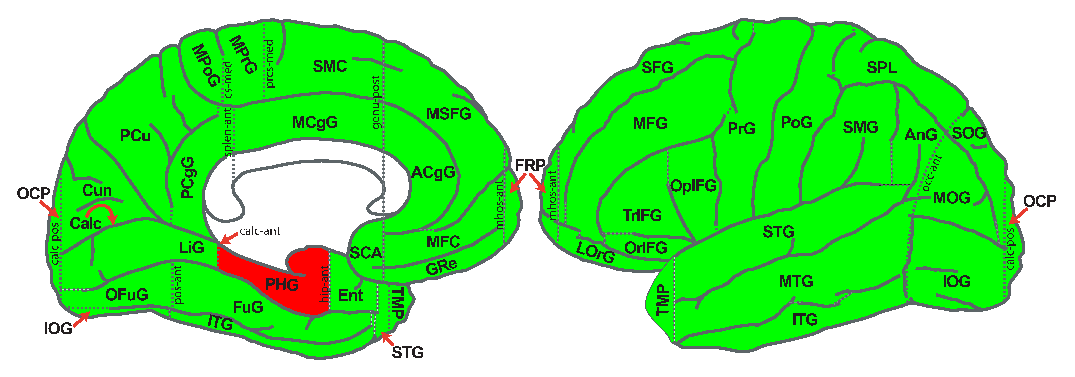
\includegraphics[scale=1]{parahippo_red.eps}
  \caption{Abnormal parahippocampal gyrus only.}
\end{figure}


\begin{figure}[H]
  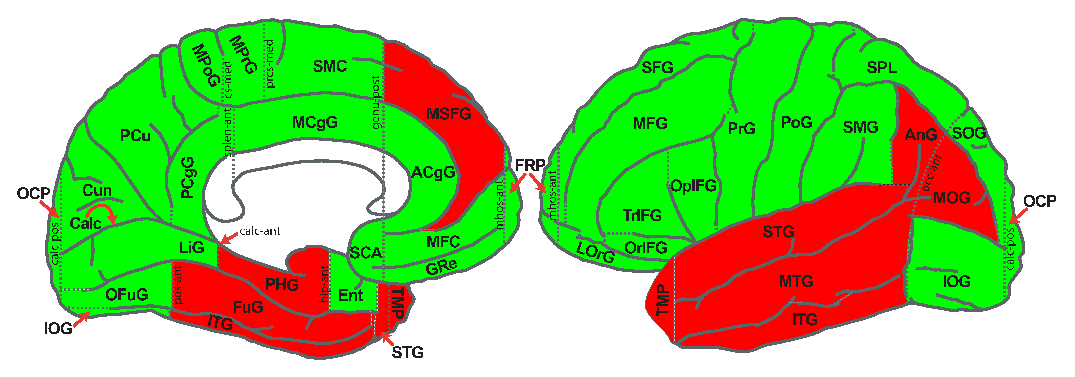
\includegraphics[scale=1]{msfg_red.eps}
  \caption{All up to MSFG abnormal. } 
\end{figure}


\begin{figure}[H]
  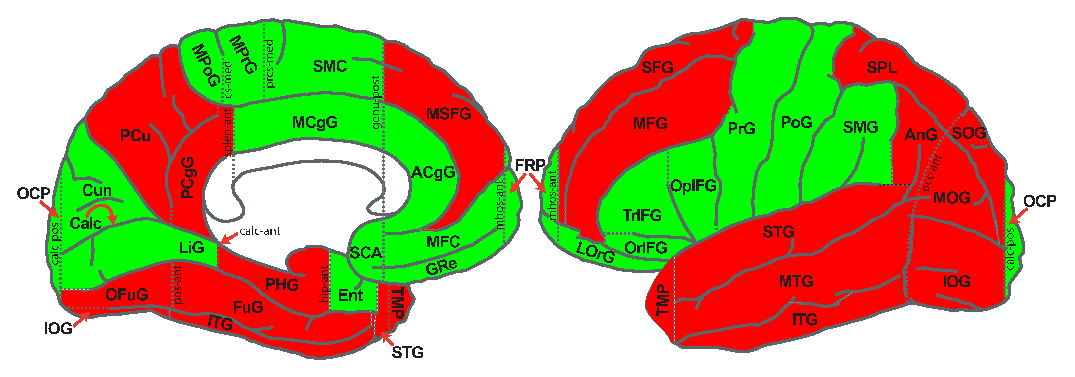
\includegraphics[scale=1]{pt_red.eps}
  \caption{All events abnormal. The green areas were not included in the EBM} 
\end{figure}

\clearpage

The following EBM events are not included in the dataset of the program:
\begin{itemize}
 \item ABETA142
 \item PTAU181P
 \item RAVLT\_immediate
 \item MMSE
 \item ADAS13
 \item Hippocampus\_TIV
 \item Amygdalia\_TIV
 \item Ententorhinal area\_TIV 
 \item vessed\_TIV
 \item FDG
 \item Cerebral exterior
 \item Inf Lat Vent\_TIV
 \item Thalamus proper\_TIV
 \item Lateral Ventricle\_TIV
 \item 3rd Ventricle\_TIV
 \item Non-ventricular CSF\_TIV
 \item Aocumbens area
 \item Ventral DC\_TIV
 \item Optic chiasm\_TIV
\end{itemize}


\end{document}
